\section{Preliminaries}
\label{sec:preliminaries}

\subsection{Data Model}
\label{sec:data-model}

A schema, denoted as \(S = (a_1, a_2, \ldots, a_n)\), is a collection of attributes. Each attribute \(a_i\) in this schema is associated with a specific data domain \(D_i\), which defines the set of permissible values that \(a_i\) can take.
A relation \(R\) is defined as a set of tuples. We consider \(R\) to be a relation over schema \(S\), if and only if, every tuple \(t = (d_1, d_2, \ldots, d_n)\) in \(R\) adheres to the schema's constraints, such that the value \(d_i\) for each position in the tuple corresponds to the data domain \(D_i\) of the attribute \(a_i\) in \(S\). In other words, each value \(d_i\) in a tuple \(t\) is drawn from the appropriate data domain \(D_i\) for its corresponding attribute \(a_i\).
Moreover, for any tuple \(t\) in the relation \(R\), the notation \(t.a_i = d_i\) signifies that the attribute \(a_i\) in tuple \(t\) has the value \(d_i\).
To formalize the integration of graph syntax within the realm of relational data, we reference the property graph model as outlined in~\cite{property-graph}. In this context, we introduce the concept of a \textit{Relations-to-Graph Mapping} (i.e. \rgmapping), to facilitate the transformation of relational data structures into a property graph.

%Given two relations, \(R_1\) and \(R_2\), each with its own schema. Let there be a bijective relation mapping, \(\lambda: R_1 \mapsto R_2 \).
\begin{definition}[\rgmapping, $\zeta$]
\label{def:rgmapping}
Given two sets of relations: \(\vec{R_v} = \{R_{v_1}, R_{v_2}, \ldots, R_{v_n}\}\) and \(\vec{R_e} = \{R_{e_1}, R_{e_2}, \ldots, R_{e_m}\}\), an \rgmapping, denoted as \(\zeta: \vec{R_v} \cup \vec{R_e} \to G\), is defined to map the relations to a property graph \(G = (V, E, \id, \lab)\)\footnote{Note that we will write $G = (V, E)$ for simplicity in the following.}, where \(V\) and \(E\) are the vertex and edge sets of \(G\), respectively. This mapping is elaborated as follows:

\begin{itemize}
\item \textbf{Vertex Mapping}: For each relation \(R_{v_i}\) in \(\vec{R_v}\), every tuple \(t\) is mapped to a unique vertex \(v \in V\). This vertex \(v\) is assigned a unique identifier \(\id(v)\), a label \(\lab(v)\) that matches the name of \(R_{v_i}\), and attributes \(v.a_i\) that mirror the attributes \(t.a_i\) of \(t\).

\item \textbf{Edge Mapping}: For the relations in \(\vec{R_e}\), each relation \(R_{e_i}\) is associated with two subsets of vertices, determined by \emph{total} functions \(\lambda_s: R_{e_i} \to R_{v_s}\) and \(\lambda_t: R_{e_i} \to R_{v_t}\), where \(R_{v_s}\) and \(R_{v_t}\) are relations in \(\vec{R_v}\). For each tuple \(t \in R_{e_i}\), a corresponding edge \(e\) is defined, linking vertices that \rgmapping maps from \(\lambda_s(t) \in R_{v_s}\) and \(\lambda_t(t) \in R_{v_t}\) as the source and target vertices, respectively. Similar to vertices, each edge \(e\) receives a label \(\lab(e)\) corresponding to the name of \(R_{e_i}\) and attributes \(e.a_i\) that reflect the attributes of \(t\).

\end{itemize}
\end{definition}

\todo{refine examples}

\comment{
Let $L$ and $T$ be finite sets of labels and types respectively, $D = \bigcup_i D_i$ be the union of atomic domains $D_i$, and $\epsilon$ be the \kw{NULL} value. We define a \textit{property graph} as $G = (V, E, \lambda, L, T, \vlabel, \elabel, P_v, P_e)$, where
\begin{itemize}
    \item $V$ is a finite set of vertices,
    \item $E$ is a finite set of edges,
    \item $\lambda: E \mapsto V \times V$ connects each edge $e$ with a tuple $(s, t)$ of source and target vertices,
    \item $\vlabel: V \mapsto 2^L$ assigns a set of labels to each vertex,
    \item $\elabel: E \mapsto T$ assigns a type to each edge,
    \item $P_v$ is a set of vertex properties, where $p_v^i: V \mapsto D_i \cup \{\epsilon\}$ is a partial function that assigns a property value in $D_i$ to each vertex.
    In particular, if a vertex $v$ does not have the property $p_v^i$, $p_v^i(v) = \epsilon$,
    \item $P_e$ is a set of edge properties, where $p_e^j: E \mapsto D_j \cup \{\epsilon\}$ is a partial function that assigns a property value in $D_j$ to each edge.
    In particular, if an edge $e$ does not have the property $p_e^j$, $p_e^j(e) = \epsilon$.
\end{itemize}
For simplicity, vertices and edges are collectively referred to as graph elements.
Given a vertex $u \in V$, we write $u.prop$ to access the value of property $prop$ of $u$, and it is analogous for edges.




The attributes of $S$ is denoted as $\attr(S) = U$. The value of each attribute $a \in \attr(S)$ comes from specific domain, denoted as $\Dom(a)$.

A relation $R$ is a set of tuples, and $R$ is called to be over schema $S$ if and only if for each tuple $t \in R$, its $i$-th item (i.e., $t_i$) satisfies $t_i \in Dom(a_i)$.
A relation can be represented as a relational table \cite{relation-as-table}.
Given a property graph $G$, a graph schema is such a schema $S_g$ that $\forall a \in \attr(S_g)$, $\Dom(a) \subseteq V \cup E$.
In other words, each attribute of a graph schema is either a vertex or an edge.
A relation $GR$ over a graph schema $S_g$ (i.e. $\sch(GR) = S_g$) is called a graph relation.
% For simplicity, we denote $\attr(GR)$ in short for $\attr(S_g)$ with $\sch(R) = S$ to retrieve the attributes of a graph relation $GR$.
% We write $GR.a$ to access a given attribute $a$ in the relation $GR$.

% Given a graph relation $GR$, if $a \in \attr(GR) \subseteq V \cup E$, we can further access the property $p$ on the vertex/edge attribute via $p(GR.a)$ (or $p(a)$ if the graph relation $GR$ is clear in the context).
% Particularly, we use $\id$ and $\lab$/$\type$ to denote the built-in properties of the globally unique identifier and label/type of a vertex/edge.
To clarify ambiguity, the term ``attribute'' always refers to the attribute of a relation or a graph relation, while the term ``property'' always refers to the property of a graph element in this paper.

\begin{definition}[RG Mapping, $\zeta$]
    Given a set of relations $SR$, an RG mapping $\zeta_{V_r, E_r, \mathcal{C}}$ maps $SR$ to a property graph $G = \zeta_{V_r, E_r, \mathcal{C}}(SR)$, where $V_r$ and $E_r$ are two subsets of $SR$ with $V_r \cap E_r = \emptyset$.
    $\mathcal{C}$ is a set of 7-tuples $(e_n, e_{scol}, e_{tcol}, v_{sn}, v_{scol}, v_{tn}, v_{tcol})$, where $e_n$ is the name of a relation in $E_r$, $e_{scol}$ and $e_{tcol}$ are attributes of that relation.
    Similarly, $v_{sn}$ and $v_{tn}$ are names of relations in $V_r$, $v_{scol}$ and $v_{tcol}$ are attributes of these two relations respectively.
    The resultant property graph $G$ satisfies that
    (1) Each vertex $u \in G.V$ corresponds to a row of a table in $V_r$, the label of $u$ equals the name of the table, the properties of $u$ corresponds to the attributes of the row.
    (2) Each edge $e \in G.E$ corresponds to a row of tables in $E_r$, the label of $e$ equals the name of the table, the properties of $u$ corresponds to the attributes of the row;
    (3) Given $(e_n, e_{scol}, e_{tcol}, v_{sn}, v_{scol}, v_{tn}, v_{tcol}) \in \mathcal{C}$, $\forall e \in G.E$ with $\elabel(e) = e_n$, $\exists u_1, u_2 \in G.V$ with $\vlabel(u_1) = v_{sn}$ and $\vlabel(u_2) = v_{tn}$, we have $e_n.e_{scol} = u_1.v_{sn}$ and $e_n.e_{tcol} = u_2.v_{tcol}$.
\end{definition}

A set of relations can be transformed to a property graph with an RG mapping.
Clearly, a property graph $G$ can be further transformed to a graph relation by constructing a tuple consisting of the vertices and edges in $G$.
Then, a graph relation containing the tuple is generated.
}

\begin{example}
    According to the grammar of SQL/PGQ, an RG mapping is defined with the \lstinline{CREATE PROPERTY GRAPH} statement.
    For instance, an RG mapping is presented as follows.
    \begin{lstlisting}
        CREATE PROPERTY GRAPH graph_view
            VERTEX TABLES (
                Person PROPERTIES(person_id, name),
                Message PROPERTIES(message_id, content)
            )
            EDGE TABLES (
                Send SOURCE KEY(pid) REFERENCE Person(person_id) DESTINATION KEY(mid) REFERENCE Message(message_id)
            )
    \end{lstlisting}
    Specifically, $V_r = \{Person, Message\}$, $E_r = \{Send\}$, and $\mathcal{C} = (Send,$ $pid, mid, Person, person\_id, Message, message\_id)$.

\end{example}

%In the rest of this paper, let $\mathcal{J}_{GR} = 2^{2^{V \cup E}}$ be the domain of graph relations, $\mathcal{J}_R = 2^{2^{D}}$ be the domain of relations, and $\mathcal{J} = \mathcal{J}_{GR} \cup \mathcal{J}_R$.

\subsection{Relational Matching Algebra}
\label{sec:graph-relational-algebra}
Graph pattern matching lies at the core of graph query processing, and is also the most fundamental extension in SQL/PGQ~\cite{sqlpgq}.
%In this work, we extend the conventional relational algebra to equip it with the capability to handle graph pattern matching.
With \rgmapping to transform relational data into a property graph $G(V, E)$, we introduce a new algebra that can handle both relational and graph data.
Let $GR$ denote a graph relation over a schema $S = (v_1, v_2, \ldots, v_n, e_1, e_2, \ldots, e_m)$, where the domain of each $v_i$
is the vertex set $V$, and the domain of each $e_j$ is the edge set $E$ in $G$, respectively.
A graph relation \(GR\) can be seamlessly transformed into a traditional relation \(R\) via a specialized projection operator, \(\widehat{\pi}_{v_1.a_{v_1}, \ldots, e_1.a_{e_1}, \ldots}\). This operator meticulously projects each vertex and edge onto specified attributes. Consequently, the resultant relation \(R\) is fully compatible with conventional relational operations, thus enabling the integration of graph-based data within the realm of existing relational databases. %and facilitating a holistic approach to data management and query processing.


The new algebra is named relational matching algebra.
The relational matching algebra expands the domain and range of the operators in relational algebra and introduces a new operator, i.e., the matching operator.
Specifically, the inputs and outs of the operators such as selection ($\sigma_d$), projection ($\pi_A$), and join ($\Join$) operators are allowed to be relations and graph relations.
In other words, in relational matching algebra, these operators act on relations or graph relations, and their outputs are also relations or graph relations.
Since the semantics of these operators remain unchanged, the description of these operators are omitted.
The formal definition of the matching operator is as follows.

\begin{definition}[Matching Operator, $\mathcal{M}$]
    Given a graph relation $GR$ representing the data graph and a pattern $\mathcal{P}$, the matching operator takes a graph relation and a pattern as inputs, and outputs a graph relation $GR_{out}$ as the result, i.e., $\mathcal{M}(GR, \mathcal{P}) \rightarrow GR_{out}$.
    The graph relation consists of the subgraphs matching the pattern.
    % $\mathcal{M}: \mathcal{J}_{GR} \times \mathcal{Q} \rightarrow \mathcal{J}_{GR}$ returns a graph relation consisting of the subgraphs matching the pattern.
    % $\mathcal{Q}$ is the set of possible patterns.
\end{definition}

By default, the matching operator adopts the homomorphism semantics.
Therefore, in the output graph relation of the matching operator, each row is a tuple of vertices and edges, whose corresponding property graph is homomorphic to the given pattern.

A special kind of projection is graph projection that maps graph relations to relations.
%$\widehat{\pi}_{prop} : \mathcal{J}_{GR} \rightarrow \mathcal{J}_{R}$ that maps graph relations to relations.
$\widehat{\pi}_{prop}$ is always used immediately following the matching operator to map vertices and edges to their properties, respectively.


\iffalse
Please note that the matching operator adopts homomorphism semantics by default.
The matching operator is a logical concept and has varied physical implementations.
For example, by applying the selection operator to filter the input tables based on specified constraints, one can obtain tables consisting of nodes and edges with various labels.
Then, by associating these tables through hash join, homomorphic subgraphs corresponding to the pattern can be found.
Please note that the results of pattern matching can be correctly obtained through joins between tables, and it is proven in Sec.~\ref{sec:proof-gpm-gro}.
Clearly, replacing hash join with other join methods like merge join or changing the join order can yield more physical implementations of the matching operator.
\fi





\iffalse
\subsubsection{Source}
The source operator gets vertices from a graph according to the constraints specified on the labels of the vertices.

\begin{definition}
    The source operator $\bigcirc_{(v:l_1, \cdots, l_k)}$ gets a set of vertices from the graph.
    Each obtained vertex should contain the specified labels $l_1, \cdots, l_k$.
\end{definition}

\begin{figure*}
    \centering
    \begin{subfigure}[b]{0.4\linewidth}
        \centering
        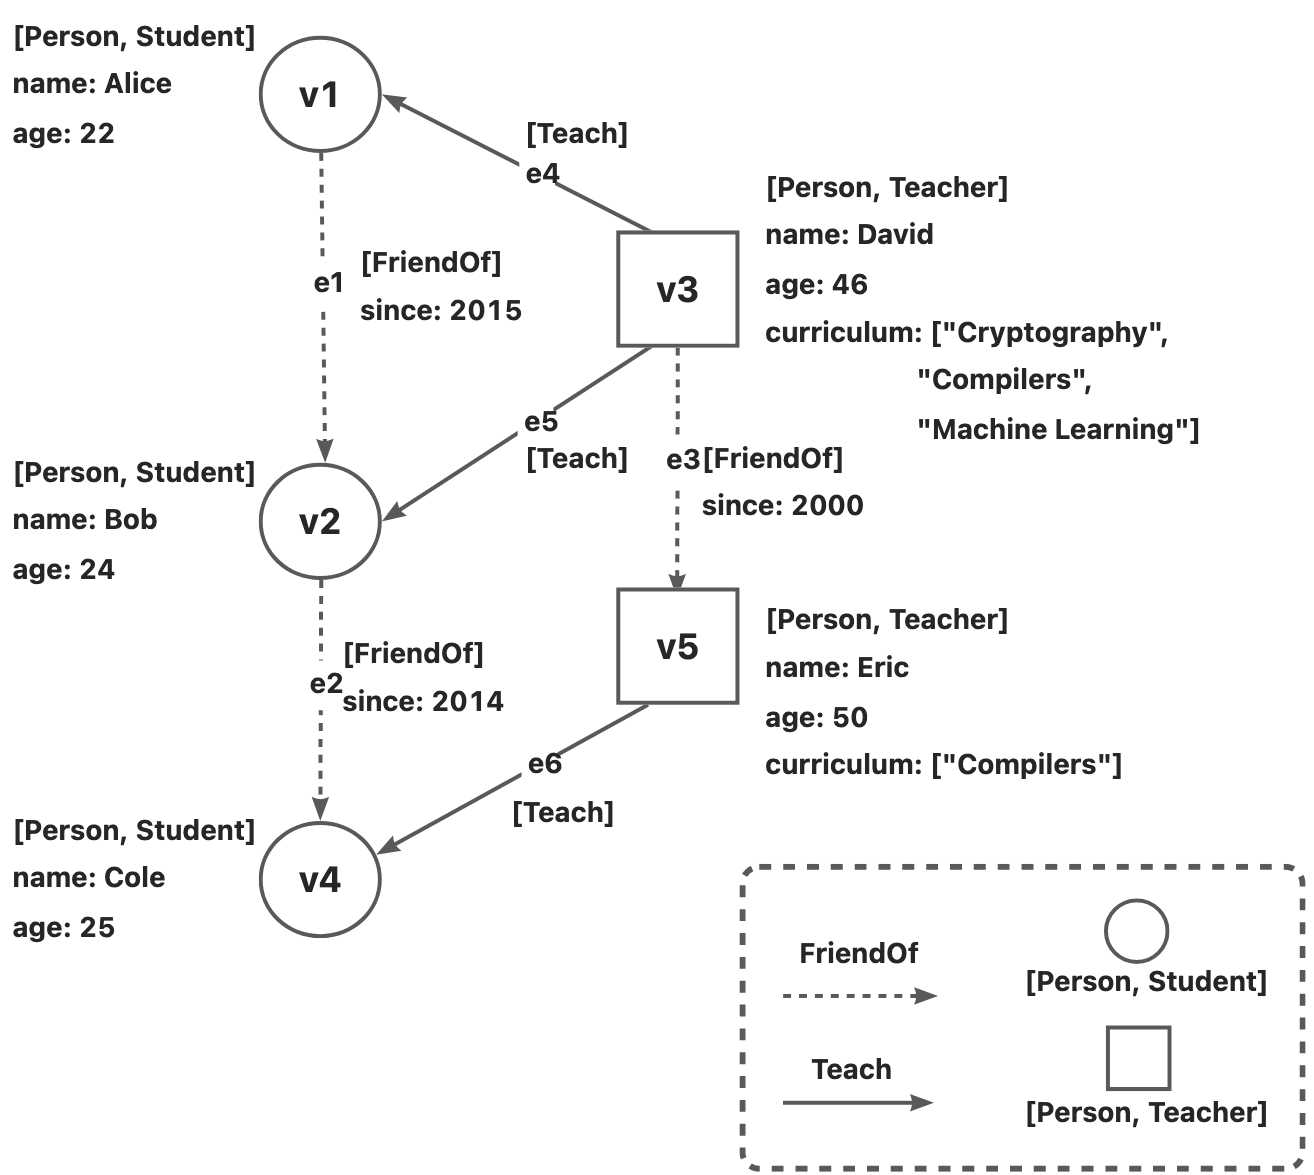
\includegraphics[width=\linewidth]{./figures/example-graph.png}
        \caption{Example Graph.}
        \label{fig:example-graph}
    \end{subfigure}
    \begin{subfigure}[b]{0.4\linewidth}
        \centering
        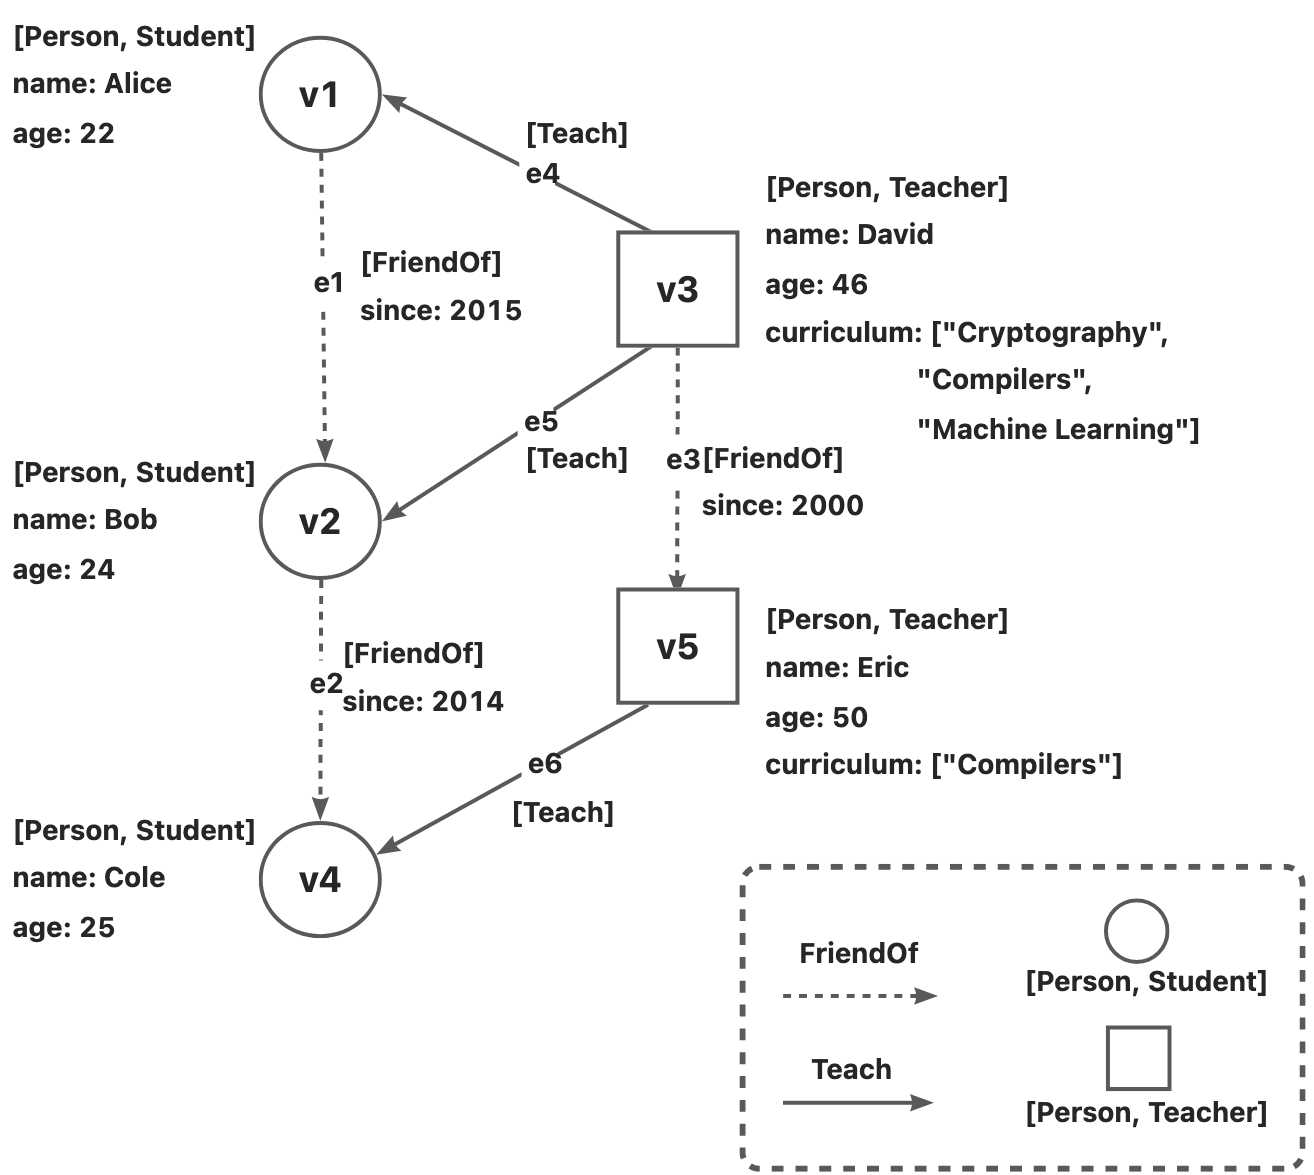
\includegraphics[width=\linewidth]{./figures/example-graph.png}
        \caption{Formal Definition of Example Graph.}
        \label{fig:example-graph-def}
    \end{subfigure}
    \caption{Definition of an example graph.}
    \label{fig:example-graph-full}
\end{figure*}

\begin{example}
    Suppose property graph $G = (V, E, \lambda, L, T, \mathcal{L}, \mathcal{T}, P_v, P_e)$ represents the relationships among persons.
    The property graph is shown in Fig.~\ref{fig:example-graph}.
    Then, to find all the persons with label \text{Student}, the corresponding expression is:
    \begin{equation*}
        \bigcirc_{(v_1\text{:Person})}.
    \end{equation*}
\end{example}


\subsubsection{Selection}

The selection operator is used to filter out the records that do not satisfy the specified constraints.
The formal definition of the selection operator is as follows.

\begin{definition}
    The selection operator is a mapping $\sigma_d : \mathcal{J} \rightarrow \mathcal{J}$, where $d$ represents the constraints the resultant records should satisfy.
\end{definition}

\begin{example}
    To find all the students whose name is ``Bob'', the following expression can be used:
    \begin{equation*}
        \sigma_{v_1.\text{name} = ``Bob''}\bigcirc_{(v_1\text{:Student})}.
    \end{equation*}
\end{example}

\subsubsection{Projection}
The projection operator bridges the gap between graphs and tables, which make it possible to combine graph and relational queries.
Its formal definition is as follows.

\begin{definition}
    The projection operator is a mapping $\pi : \mathcal{J} \rightarrow \mathcal{J}$, which maps vertices and edges to a subset of them or their properties, and maps other attributes to a subset of them.
\end{definition}

Please note that if the resultant records of a projection operator cannot contain any vertex or edge, then it is called a flatten projection operator $\hat{\pi} : \mathcal{J} \rightarrow \mathcal{J}_D$.
A flatten projection operator can convert a property graph to a relational table.

\begin{example}
    Suppose we are going to get a relational table of persons, and the schema of the table is (name, age).
    Then, the following expression can achieve the goal.
    \begin{equation*}
        \pi_{v.name, v.age}(\bigcirc_{(v:Person)}).
    \end{equation*}
\end{example}

\subsubsection{Expand}

The expand operator gets the edges adjacent to the given vertices.
Based on the direction of the expansion, the expand operator can be categorized into three types, i.e., expand-out ($\uparrow$), expand-in ($\downarrow$), and expand-both ($\updownarrow$).
For simplicity, the definition of the expand-both operator is given as follows, and those of expand-out and expand-in are similar.

\begin{definition}
    The expand-both operator is a mapping $\updownarrow_{(v)}^{(w:L)}[e] : \mathcal{J} \rightarrow \mathcal{J}$.
    For each record $c$ containing vertex $v$ and each edge $e$ satisfying $\lambda(e) = (v, w)$ (or $\lambda(e) = (w, v)$), a new record is created by appending ($e$, $w$) to $c$.
\end{definition}

\begin{example}
    To get all the ``Teaching''' relationships between students and teachers, the following expression can be used:
    \begin{equation*}
        \downarrow_{(v)}^{(v_t\text{:Teacher})}[\text{:Teaching}]\bigcirc_{(v\text{:Student})}.
    \end{equation*}
\end{example}

\subsubsection{Join}

The join operator can join two relational tables or join two property graphs.
Similar to that in relational algebra, the join operator in graph relational algebra also has many types, such as natural join ($\Join$), left-outer join, and right-outer join.
For simplicity, the definition of natural join is proposed, and those of other types of joins is similar.

\begin{definition}
    The natural join operator $\Join : \mathcal{J} \times \mathcal{J} \rightarrow \mathcal{J}$ combines two relations if they have the same values on common attributes.
\end{definition}

The natural join operator can be expressed as follows:
\begin{equation*}
    \begin{split}
        & R \Join P = \sigma_{R.a_1 = P.a_1 \land \cdots \land R.a_k = P.a_k}(R \times P), \\
        & \hspace{2em} \text{where } \text{attr(sch($R$))} \cap \text{attr(sch($P$))} = \{a_1, \cdots, a_k\}
    \end{split}
\end{equation*}

\begin{example}
    To obtain the names of the teachers who teach the common friends of Alice and Bob, the following expression can be used:
    \begin{equation*}
        \footnotesize
        \begin{split}
            & \pi_{v_3\text{.name}}( \\
            & \hspace{1em} (\downarrow_{(v_c)}^{(v_3\text{:Person})}[\text{:Teaching}]\updownarrow_{(v_1)}^{(v_c\text{:Person})}[\text{:Friend}]\sigma_{v_1\text{.name=``Alice''}}(\bigcirc_{(v_1\text{:Person})})) \\
            & \hspace{1em} \Join (\updownarrow_{(v_2)}^{(v_c\text{:Person})}[\text{:Friend}]\sigma_{v_2\text{.name=``Bob''}}(\bigcirc_{(v_2\text{:Person})}))\\
            & )
        \end{split}
    \end{equation*}
\end{example}

\subsubsection{Aggregation}
The aggregation operator groups the records according to the values of the specified attributes, and output new records that may contain aggregated values.
The aggregation operator is denoted by $\gamma_{c_1, \cdots, c_i}^{o_1, \cdots, o_j}$.
Specifically, the records are grouped according to attributes $c_1, \cdots, c_i \in V \cup E \cup D$, and $o_1, \cdots, o_j$ are the outputed new attributes.

\begin{example}
    To count the number of students taught by David, the following expression can be used:
    \begin{equation*}
        \gamma_{}^{count(v_s)}\uparrow_{(v_1)}^{(v_s:Student)}[\text{:Teaching}]\sigma_{v_1\text{.name=``David''}}(\bigcirc_{(v_1:Person)})
    \end{equation*}
\end{example}

\subsubsection{Sorting and Top}

The sort operator $\tau_{* a_1, \cdots, * a_n}$ is used to sort the input graph relation according to attributes $a_1, \cdots, a_n \in D$.
Specifically, `*' can be $\uparrow$ or $\downarrow$, representing sorting the records ascendingly or descendingly, respectively.
The results of the sort operator are put in an ordered list rather than a bag.

The top operator $\lambda_k^s$ skips the first $s$ records in the input list, and return the next $k$ records as the outputs.
Since the \emph{bag} semantics are applied in graph relations, the records are unsorted by default and the top operator is meaningless in such bags.
Therefore, the sort operator is usually applied before the top operator is used.

\begin{example}
    To obtain the most aged five teachers, the utilized expression can be as follows:
    \begin{equation*}
        \lambda_{0}^{5}\tau_{\downarrow \text{age}}(\bigcirc_{(v_1\text{:Teacher})})
    \end{equation*}
\end{example}


\subsubsection{Unwind}

Given a graph relation $R$, suppose attribute $xs \in \text{attr}(\text{sch}(R))$ is a list.
Then, for each record $r$ in $R$, the unwind operator appends each value in $r.x$ to $r$ respectively and removes attribute $xs$ from $r$ to generate new records.
The formal definition of the unwind operator is as follows.

\begin{definition}
    Given graph relation $R$ with $\text{sch}(R) = (a_1, \cdots, a_n)$.
    Without loss of generality, suppose the value of attribute $a_1$ is of list type.
    Then, we have $\text{sch}(\omega_{a_1 \rightarrow a_s}(R)) = (a_2, \cdots, a_n, a_s)$.
    For each record $(val_1, \cdots, val_n) \in R$ with $val_1 = [l_1, \cdots, l_k]$,  $k$ new records are generated, where $r'_j = (val_2, \cdots, val_n, l_j)$, $j \in \{1, \cdots, k\}$.
\end{definition}

\begin{example}
    To get all the classes taught by David, the following expression can be used:
    \begin{equation*}
        \begin{split}
            \pi_{\text{course}}(\omega_{\text{curriculum} \rightarrow \text{course}}(\sigma_{v_1\text{.name=``David''}}(\bigcirc_{(v_1\text{:Person})}))).
        \end{split}
    \end{equation*}
\end{example}

\subsubsection{Match}

Given two graph relations $V$ and $E$ representing the vertex table and edge table of a graph respectively and a pattern $\mathcal{P}$, mapping $\mathcal{M}: \mathcal{J} \times \mathcal{J} \times \mathcal{Q} \rightarrow \mathcal{J}$, where $\mathcal{Q}$ is the set of possible patterns.

The match operator adopts homomorphism semantics by default.

According to SQL/PGQ, the outputs of graph queries should be a relation consisting of property values, identifiers, labels or types.
References to vertices or edges should not be returned by graph queries.
Therefore, the outputs of the graph relational algebra are projected and flattened with the project and unwind operator, respectively.
Then, the output graph relation is converted to a relation over a relational schema, and can be involved in the following optimization of relational optimizer.
\fi

\subsection{Problem Definition}
\label{sec:problem-definition}

Select-Project-Join (abbr.~SPJ) queries are widely utilized in previous studies \cite{spj} and are defined as follows:
\begin{equation*}
    Q = \pi_A(\sigma_d(R_1 \Join \cdots \Join R_m)).
\end{equation*}
Specifically, SPJ queries describe a \emph{pattern} with the linear sequence of join operators.
Inspired by SPJ queries, for the property graph data model proposed in Sec.~\ref{sec:data-model}, we design a new class of queries named SPJM under relational matching algebra.
The definition of an SPJM query is as follows:
\begin{equation*}
    Q_m = \pi_A(\sigma_d(R_1 \Join \cdots \Join R_m \Join \widetilde{R}_1 \Join \cdots \Join \widetilde{R}_n))
\end{equation*}
where
\begin{equation*}
    \tilde{R}_i = \hat{\pi}_{prop_i}(\mathcal{M}(GR_i, \mathcal{P}_i))
\end{equation*}
is a relation generated by projecting the outputs of the matching operator $\mathcal{M}$ to relations of properties.
Besides, $GR_i$ is the graph relation that contains the data graphs that pattern matching is conducted on and $\mathcal{P}_i$ is the pattern.
$prop_i$ is a list of necessary properties of vertices and edges in the resultant relation.

\iffalse
Regarding the SPJM problem, the main difference between the aforementioned four types of optimizers lies in their search space when optimizing the physical implementation of the matching operator.
Specifically, for $Rel$ methods, the matching operator is implemented with only joins that do not leverage graph indices (named relational joins) such as hash joins.
Therefore, $\widetilde{R}_i$ can be optimized with the relational optimizer.
For $Rel^+$ methods, in the process of optimization, the matching operator is implemented with relational joins.
Thus, the relational optimizer is also utilized to optimize $\widetilde{R_i}$.
However, after that, relational joins are replaced with joins that leverage graph indices (named graph joins) if possible such as sip join in GrainDB.
For $Rel+G$ methods, graph joins are considered in implementing the matching operator.
Then, operators inside of $\widetilde{R}_i$ are optimized by the graph optimizer, while the operators out of $\widetilde{R}_i$ are optimized by the relational optimizer.
Besides, the optimizations cannot be simultaneously related to operators within and outside of $\widetilde{R}_i$.
For example, the filter operators, i.e., $\sigma_d$ cannot be pushed into $\widetilde{R}_i$.
For $Rel\&G$, such optimizations are allowed.
\fi

% The search space for relgo in the context of a SPJG query consists of operator trees that correspond to sequence of join operators, e.g., the sequence
% \begin{lstlisting}
%     Join(Join(Join(Join(GR_1, GR_2), R_1), R_2), R_3)
% \end{lstlisting}


\iffalse
\subsection{Equivalence Between Graph Pattern Matching and Graph Relational Operators}
\label{sec:proof-gpm-gro}

For the SPJG problem to be solved in this paper, we need to obtain the graph relations by pattern matching.
In detail, the pattern matching process ought to be expressible through the traversal of paths, which are sequences of source, expand, and join operators.
In this section, we prove that the match operator can be replaced with source, expand, and join operators. without changing the semantics of the query.
Then, the matching order can be further optimized by relgo.

We start from the case that there is only one path in the specified pattern, and firstly, we focus on homomorphic pattern matching.
Then, we have the following theorem.

\begin{theorem}
    Homomorphic pattern matching with a path pattern can be expressed with graph relational algebra expressions.
\end{theorem}
\begin{proof}
    The graph relational algebra operators related to pattern matching include source, expand, join, and extend-intersect.
    Then, we prove the theorem by induction.
    Let each vertex and edge in a path pattern be an element.
    If for each edge in a pattern, its adjacent vertices are also specified in the pattern, then the pattern is called a strict pattern $P$.
    Otherwise, it is a loose pattern $\hat{P}$.

    %Since path patterns specified in SQL/PGQ are all strict patterns are, the induction is conducted on the number of elements in the strict pattern.
    The path pattern is a strict pattern, and induction is conducted on the number of elements in the strict pattern.
    When there is only one element (i.e., a vertex like ``(u:Label)'') in the pattern, the corresponding algebra expression of the pattern is $\bigcirc_{(u:\text{Label})}$, and it is clear that the expression equals the pattern.

    Then, suppose for a path pattern with at most $n$ elements, the corresponding algebra expressions have the same meaning as matching the path pattern.
    Denote a graph relational algebra with the same meaning as matching path pattern $P$ by $E_p$.

    When there are $n + 1$ elements in the path pattern $P$:

    %Condition 1: $P = P_1, P_2$, i.e., pattern $P$ is obtained by concatenating subpatterns $P_1$ and $P_2$.
    %(e.g., $P_1 = (u)-[e]-(v), P_2 = (u)-[e']-(w), P = (u)-[e]-(v), (u)-[e']-(w)$).
    %Then, $E_{p_1} \Join E_{p_2}$ equals $P$, since join operator implemented in relational databases follows the semantics of homomorphism.


    Condition 1: $P = P_1 - \hat{P}_2$.
    Without loss of generality, suppose vertex $v$ in $P_1$ is adjacent to an edge in $P_2$.
    (e.g., $P_1 = (u)-[e]-(v), P_2 = [e']-(w), P = (u)-[e]-(v)-[e']-(w)$).
    Then, let $P_3 = (v)-\hat{P}_2$, and the corrsponding algebra expression of $P$ can be $E_{p_1} \Join E_{p_3}$.
    $E_{p_1} \Join E_{p_3}$ equals $P$, since join operator implemented in relational databases follows the semantics of homomorphism.
    Moreover, if $\hat{P}_2$ only consists of one vertex and an edge adjacent to it (i.e., $\hat{P}_2 = [e:eLabel]-(v_t:vLabel)$).
    Then, the corresponding algebra expression of $P$ can also be $\updownarrow_{(v)}^{(v_t:vLabel)}[e:eLabel]E_{p_1}$.
    The expand operator is also implemented by joining relational tables, which follows the semantics of homomorphism.

    Condition 2: $P = P_1$ extends $v$ through edges $[e_1:eLabel1], \cdots [e_k:eLabelk]$ ($k \geq 1$), i.e., at least one vertex in $P_1$ connects to vertex $v$.
    Then, the corresponding algebra expression of $P$ is
    \begin{equation*}
        E_{p_1} \Diamond_{v_1, \cdots, v_k}^{eLabel1, \cdots, eLabelk} \bigcirc_{(v:vLabel)}.
    \end{equation*}
    Since the extend-intersect operator is implemented with relational joins and follows the semantics of homomorphism, the algebra expression has the same meaning as matching the path pattern.

    In conclusion, the corresponding algebra expressions of path pattern $P$ with $n + 1$ elements have the same meaning as matching the path pattern.

    In conclusion, adopting the homomorphism semantics, matching path patterns has the same meaning as the corresponding graph relational algebra expressions.
\end{proof}

When the match operator adopt the isomorphic semantics, it is straightforward to add some constraints with selection operators to get the graph relational expressions equal to the match operator.
Furthermore, when there are more than one path specified in the pattern, the expressions for different paths can be connected with join operators and the obtained expressions equal to the match operator.


Besides the WALK mode by default, when the path patterns are in TRAIL, ACYCLIC, or SIMPLE mode, we still have the same conclusions.
Specifically, in TRAIL, ACYCLIC, or SIMPLE mode, a selection operator needs to be added to remove the results with repeated edges or vertices.
In detail, the selection operator should wrap the corresponding algebra expression of path patterns in the WALK mode.
For example, in the TRAIL mode, the corresponding graph relational algebra expression of $P = P_1 - P_2$ is $\sigma_{c}(E_{p_1} \Join E_{p_2})$ or $\sigma_{c}(\updownarrow_{(v)}^{(v_t:vLabel)}[e:eLabel]E_{p_1})$, where $c$ is the condition specifying that every two different pattern edges bind to different edges in each result.
In the ACYCLIC and SIMPLE mode, condition $c$ should be specified according to the constraints of the mode.

Furthermore, there may be more than one path patterns specified in the <Pattern> part of SQL/PGQ queries, and the different path patterns may have different path modes.
Denote the path patterns by $P_1, \cdots, P_k$.
According to SQL/PGQ, the binding results of different path patterns are joined together.
If the match mode in SQL/PGQ is set to \textbf{REPEATABLE ELEMENTS}, there is no more constraint, and ``MATCH $P_1, \cdots, P_k$'' has the same meaning as $P_1 \Join \cdots \Join P_k$, both of which have the semantics of homomorphism.
Otherwise, if the match mode in SQL/PGQ is set to \textbf{DIFFERENT EDGES}, the same edge cannot bind to different variables in different path patterns.
Therefore, a selection operator is needed, and ``MATCH $P_1, \cdots, P_k$'' has the same meaning as $\sigma_{d}(P_1 \Join \cdots \Join P_k)$, where $d$ is the condition specifying that each edge cannot bind to more than one variables across all path patterns.
\fi
